%\begin{figure}[t!]
%	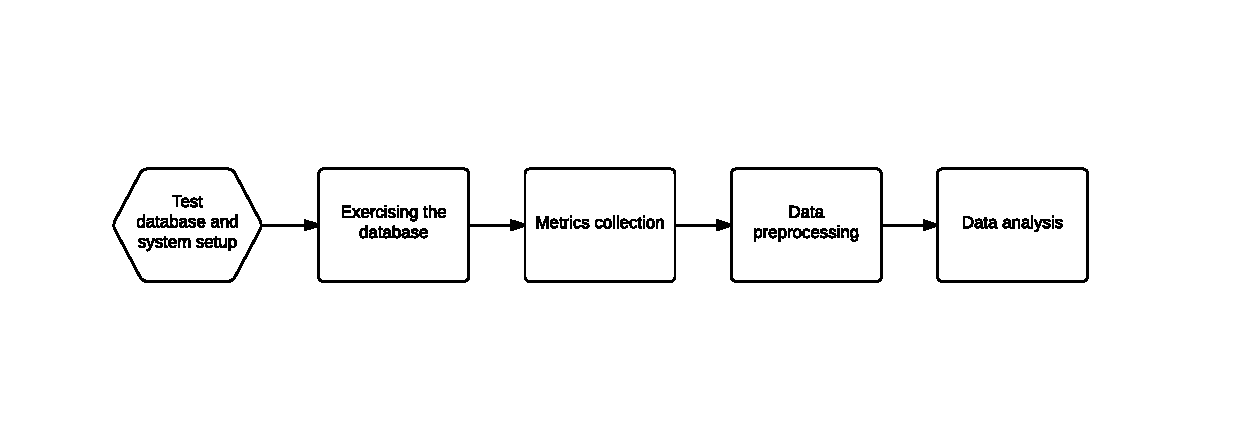
\includegraphics[width=1\textwidth]{approach.pdf}
%	\centering
%	\caption{Approach overview}
%    \label{fig:approach}
%\end{figure} 
%%\includepdf][pages={1}][width=\columnwidth{approach.pdf}

\begin{figure*}[thb]
	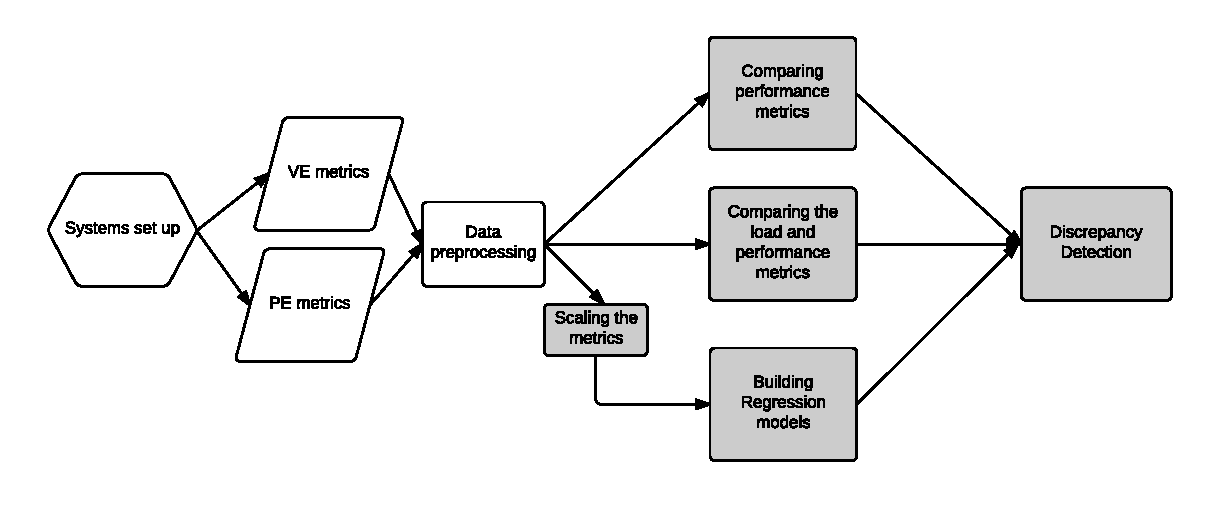
\includegraphics[width=\textwidth]{figures/approach_perf_vr1}
	\caption{Approach Overview}
	%\captionsetup{justification=centering}
	\label{fig:Approach}
\end{figure*}

In this section we discuss the steps in our approach. The primary intention behind our experiment was to observe the performance of the system under test in a virtual environment. Additionally, to analyze whether the metric values depict a similar behavior when compared cross-environment. Once the performance metrics are recorded and processed, we then analyze our results using graphical techniques and regression models. Figure 1 shows the synopsis of our approach.


\subsection{Subject Systems}
Dell DVD Store (DS2) \cite{delldvd} is an online e-commerce web application with a multitier architecture, consisting of scripts for MySQL Server and \textit{PHP} web pages. \cite{Shang:2015:ADP:2668930.2688052} \cite{Nguyen:2012:ADP:2188286.2188344}. \textit{WAMP} \cite{wamp} web application server were used to deploy the system while the database was set up on MySQL Server 5.6 \cite{mysql}. DS2 has a load driver program which is designed to exercise the system for performance testing.

CloudStore\cite{cloudstore}, our second subject system under test was also an open source application. It is a performance benchmark, based on TPC-W standards \cite{tpcw}, originally proposed by the Transaction Processing Performance Council. Just like DS2, CloudStore serves as an online ebook store, CloudStore is used as a standard in the domain of cloud computing. We deployed CloudStore on \textit{Apache Tomcat} \cite{tomcat} and MySQL Server 5.6 \cite{mysql} was used to set up the database. The workload generator was based on scripts written for Apache Jmeter. \cite{apachejmeter}

\subsection{Environmental Setup}
Our system setup included three machines in a lab environment, Intel i5 each with 8GB of memory. The first machine was dedicated to the database server, the second machine was dedicated to the web server and the third machine was used to run the load driver.
\subsubsection{Physical Setup}
To make the systems' configuration identical prior to exercising the subject systems, we chose 2 cores and 3GB of memory dedicated to each environment to avoid crashes on the guest operating system in the virtual environment. We also made sure to kill all the processes before we start our performance testing to minimize any discrepancy present.
\subsubsection{Virtual Setup}
Our virtual setup was identical to our physical setup. The virtual environment was run on the same physical machines with all the resources provided to the host and the same set of aforementioned configuration for the virtual environment. We opted for single tenancy of the guest operating system to avoid any unwanted noise. 

%\subsection{Exercising the database}
%Following the set up of our subject systems on the respective servers, the systems were exercised with an aid of drivers. These drivers generated multi-type web requests and simulated real-time user behavior depending on the input parameters provided. We ran our performance tests for numerous hours while recording all the performance metrics generated for varying load applied on our software systems.

The load variation for the drivers per run was introduced by the number of threads. A higher number of threads represented a higher number of users which would resultantly increase the number of requests per minute and vice-versa. We ran each of our test for 9 hours. The choice of load was random but consistent between both of the environments. As our study was based on exercising our systems and recording the performance metrics, and not stress testing \cite{stresstesting}, the respected limits were chosen in order to avoid the under-performance of the physical machine and system failure of the virtual machine.



%\subsection{Metrics Collection}
\subsection{Data Collection}
\subsubsection{Performance Metrics}
We used \textit{Perfmon}\cite{perfmon} to record the values of all the available performance metrics, recorded every 10 seconds. \cite{windowsperfmon}\cite{perfmon}. \textit{Perfmon} is a performance monitoring tool used to observe and record performance metrics such as CPU utilization, Memory usage and disk IOs. Our web server and database server were deployed on machines, we recorded two datasets from two application processes. Respectively, our dataset consisted of total 56 performance metrics for each performance test. The average of every six recorded entries was considered as the metric value of a minute. A set of every 6 recorded entries averaged out was labeled as a \textit{single run} representing a minute. We also removed the first and last 15 minutes to remove any kind of discrepancies present in our dataset.
\subsubsection{Throughput}
We used web server access logs to calculate the throughput of the system by measuring the requests per minute. The two data sets were then concatenated and mapped against requests according to the timestamps.

